
Understanding the composition and structure of galaxies, and the role that dark matter plays in their organization, is a pressing topic in modern cosmology. A common method to explore these questions is using numerical simulations. This approach allows us to choose plausible initial conditions and laws of physics in order to test how the universe would behave under those conditions. We can then compare those results to real-world observations to determine the accuracy of those physical assumptions. For instance, if we wanted to test Newton's theory of gravity in our solar system, we could run a numerical simulation of Newton's equation using a known initial position of the planets, and test whether the simulated motion of the planets aligns with reality. Likewise, we can test our theories about dark matter and gravity by running cosmological simulations.

\section{Physical models}

Our current leading theory for dark matter's role in galaxy evolution is the cosmological constant plus cold dark matter (\lcdm) model \citep{salesBaryonicSolutionsChallenges2022}. This theory provides a framework for cosmological simulations that incorporates a non-interacting model for dark matter and the cosmological constant model of dark energy. The "cold" dark matter model means that we assume that dark matter particles interact with neither each other nor "normal" baryonic matter, except through gravity. This is in contrast to other competing theories such as superfluid dark matter, which interacts with itself to form a superfluid \citep{delucaSuperfluidDarkMatter2023}. These dark matter models predict large dark matter halos around galaxies \citep{feldmannFIREboxSimulatingGalaxies2022}, which is consistent with observations of gravitational lensing---visual distortions due to gravity. Not much is known about dark matter beyond its gravitational effects on baryonic matter, and we have yet to find a non-gravitational interaction between these two.

The \lcdm\space assumes dark energy to be the cosmological constant $\Lambda$, which is a degree of freedom in in the Einstein Equation that adds a net offset to the energy density of a vacuum. However, there are alternative theories of dark energy; \cite{bassiCosmologicalEvolutionBimetric2023} shows that the Bimetric gravity model could also explain the effects of dark energy. If more evidence can be found in support of these alternative models, then Bimetric and/or superfluid dark matter may replace \lcdm\space as the leading cosmological model.

When creating a cosmological simulation, astrophysicists must also incorporate baryonic processes, the physics of ordinary matter. These processes include chemistry, thermal physics, and the formation, evolution, and feedback of stars. Our current computers limit us such that we cannot resolve individual stars within galaxies \citep{feldmannFIREboxSimulatingGalaxies2022} because there are simply too many, and stellar physics at these scales is not fully understood. Earlier simulations, such as \cite{bournaudISMPropertiesHydrodynamic2010}, were forced to ignore stellar processes entirely in favor of gaseous ones. They found that the simulated galaxies grew too massive and cooled too quickly compared to real galaxies. This tension was resolved by the creation of the Feedback in Realistic Environments (FIRE) physics model \citep{hopkinsFIRE2SimulationsPhysics2018}. FIRE adopts a subgrid model that simulates large chunks of matter (referred to as particles), each containing many stars. It then uses the estimated number of stars in each particle to simulate stellar feedback. 

\section{Low-mass galaxies and their tensions}
% TODO: should I always replace "dwarf" with "low mass"
Until recently, low-mass "dwarf" galaxies have not been closely studied due to them being difficult to detect with telescopes. For a period of time, the \lcdm\* model was questioned because it predicted the existence of many more dwarf galaxies than had been observed in the region around the Milky Way \citep{salesBaryonicSolutionsChallenges2022}. According to \cite{salesBaryonicSolutionsChallenges2022}, enough dwarf galaxies have been discovered in recent years to resolve this tension. However, the sudden influx of dwarf galaxy observations has provided astrophysicists number of new tensions. The diversity of the size-mass relation of dwarf galaxies is one such tension. Observational data of dwarf galaxies near the Milky Way suggests that the correlation between the mass and size of satellite dwarf galaxies is not as strong as simulations seem to predict \citep{salesBaryonicSolutionsChallenges2022}. 

\begin{figure}
    \centering
    \includegraphics*[width=\textwidth*2/3]{figs/sales/fig4.pdf}
    \label{fig:sales-size-mass}
    \caption{
        From: \cite{salesBaryonicSolutionsChallenges2022}. A comparison of the sizes and masses of dwarf galaxies from simulations and reality. The y axis plots $r_{50}$ and the x axis plots $M_{50}$. The gray squares depict real galaxies from the Milky Way's local group, whose data was compiled by \cite{mcconnachieOBSERVEDPROPERTIESDWARF2012}. The other colors depict data from various simulations other than FIREbox. As we can see, the dwarfs from the local group show much diversity in their size-mass ratios. The simulated galaxies, however, show more consistency, especially when compared to others from their own simulation (for example, notice that the orange circles are all clustered together).
        % TODO: is this tension resolved in firebox?
        % TODO: cite other papers?
    }
\end{figure}

\section{@Profe Moreno, should delete this section, or should I rewrite it?}
It is a common myth that if we can simulate something, we must be able to fully understand it. Unfortunately, this is not generally true. The galaxy simulations we use are so complex and detailed that it is often very difficult to determine what physical assumptions or initial conditions cause certain behaviors. While it is much easier to make collect data from simulations---we do not need telescopes and we can view the galaxies in 3D with arbitrary resolution---we must still analyze that data using similar techniques used to study real galaxies.

If it is demonstrated that one of these tensions is caused by neither numerical approximations in the simulations nor simplifications of baryonic physics, then it could call the \lcdm\* model into question.

%TODO: better place for this section?

\section{Tension in the size-mass relation}

% DEFINE milky way
The observed dwarf galaxies near the Milky Way have widely varying radii compared to their masses. In other words, both diffuse and compact dwarf galaxies are relatively common. However, galaxy simulations including \cite{fittsFireFieldSimulating2017} tend to form galaxies with much stricter size-mass ratios \citep{salesBaryonicSolutionsChallenges2022}. Some may argue that these discrepancies are caused by numerical inaccuracy. However, even the simulations with the highest numerical resolution such as \cite{wheelerBeItTherefore2019} lack diversity in size-mass ratios for dwarf galaxies. 

The diversity of sizes of dwarf galaxies must therefore be caused by something else. Tidal disruption could be the answer. When a dwarf galaxy passes by a larger galaxy, its dark matter halo can be destroyed by the tidal force exerted on it, according to \cite{morenoGalaxiesLackingDark2022}. This can also lead to the creation of an ultra-compact dwarf \citep{applebaumUltrafaintDwarfsMilky2021}, because the galaxy will lose its outer regions. It is therefore plausible that close interactions between galaxies is what causes variance in size.

\section{FIREbox Galaxy Simulation}
Scale and resolution are important for simulations. Astrophysicists must balance large volume and high detail, both of which cost computing power. The large volume simulations allow us to closely study intergalactic systems and to collect large amounts of statistical information about galaxies \citep{feldmannFIREboxSimulatingGalaxies2022}. However, a higher resolution "zoom in" simulation such as FIRE in the Field \citep{fittsFireFieldSimulating2017} allows us to better simulate the internal physics of the galaxies themselves.

This paper will examine data from FIREbox \citep{feldmannFIREboxSimulatingGalaxies2022}. This cosmological simulation does not have the largest volume, nor is it the most detailed. Rather, it incorporates a balance of high detail and large scale (see figure \ref{fig:feldmann-dynrange}), which together give it the highest dynamical range of any cosmological simulation to this date.



\begin{figure}
    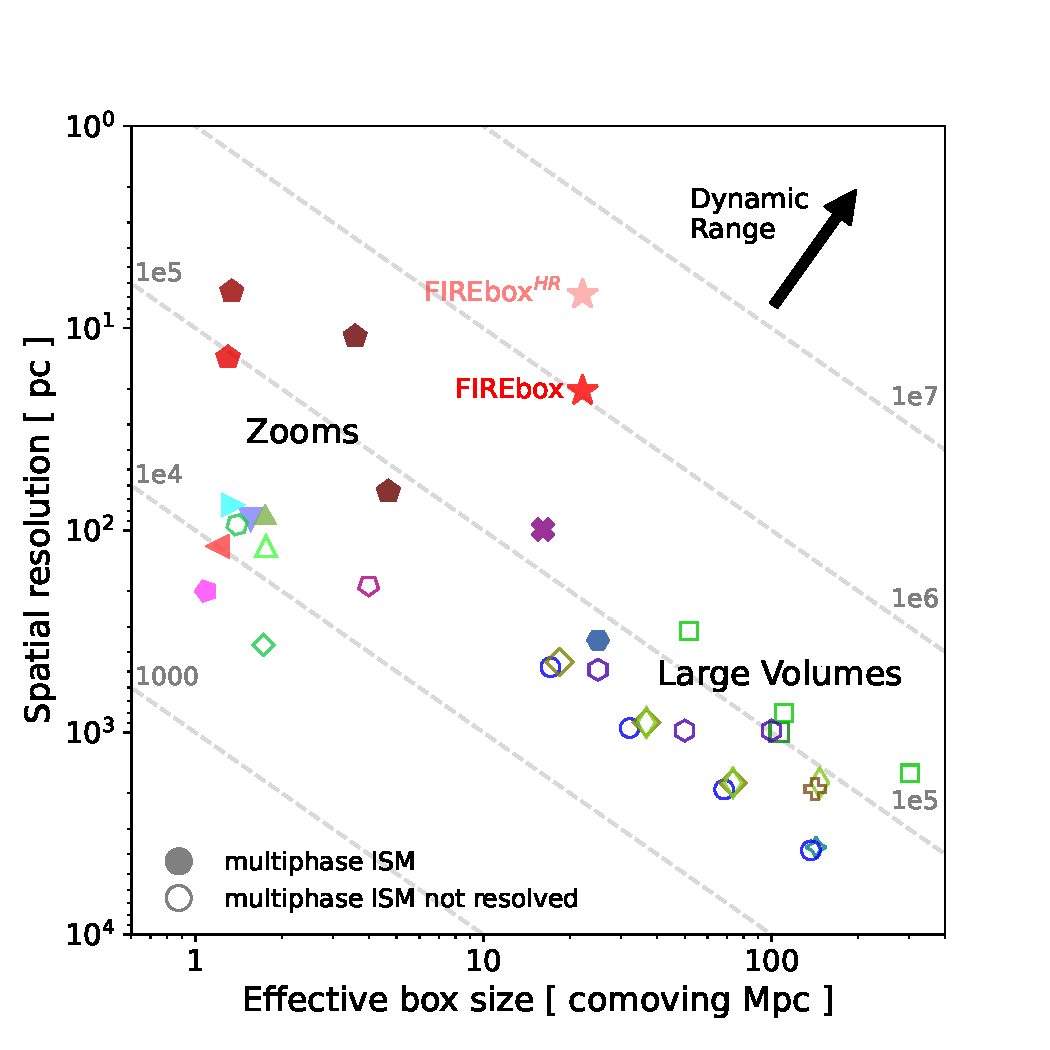
\includegraphics[width=\textwidth/2]{figs/feldmann/fig2a}
    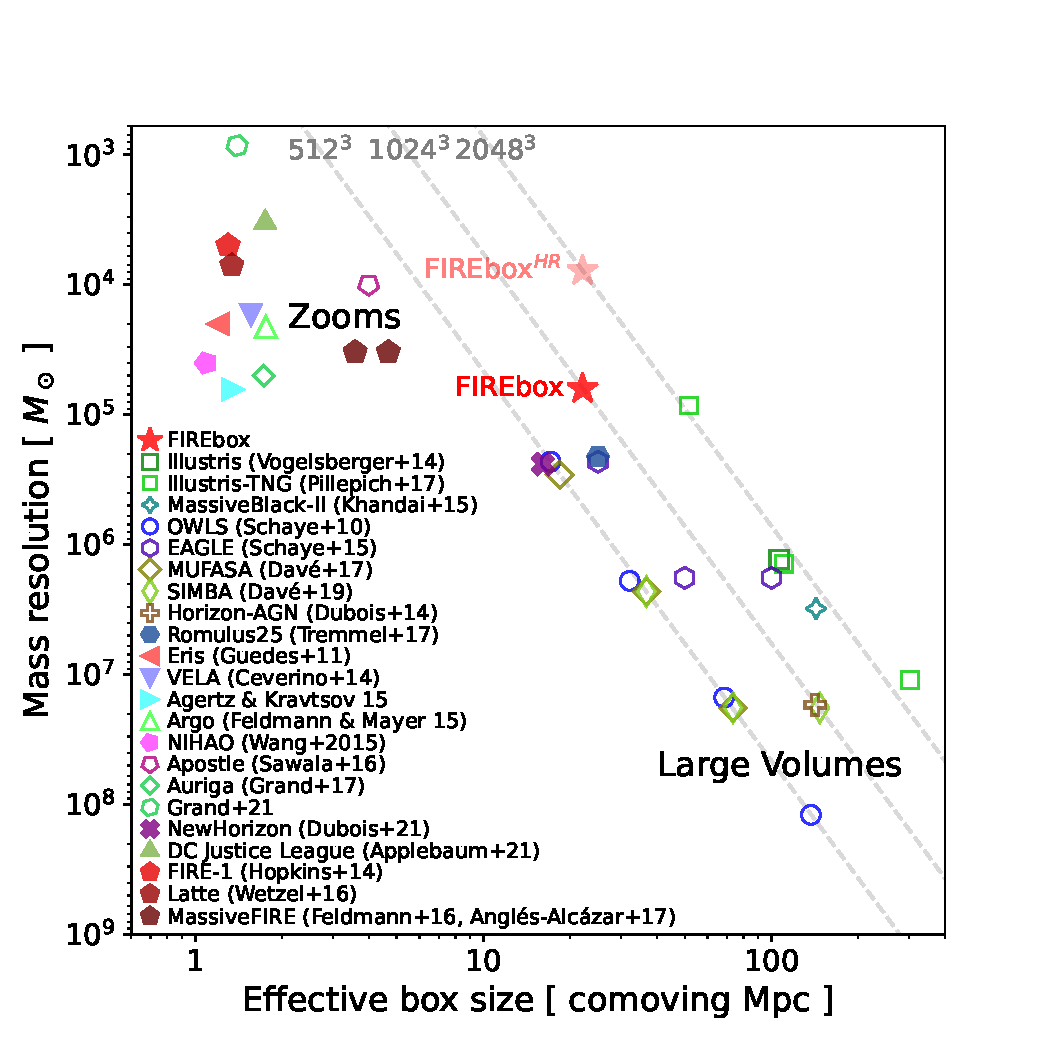
\includegraphics[width=\textwidth/2]{figs/feldmann/fig2b}
    
    \caption{A comparison the size and detail of cosmological simulations. There is a tradeoff between scale and resolution, where a total increase in both means a higher dynamic range at the cost of computer performance. FIREbox has the highest dynamic range, and therefore the highest computational cost.}

    \label{fig:feldmann-dynrange}
\end{figure}